\documentclass[12pt, usenames, dvipsnames, table]{beamer}
\usetheme{Boadilla}
\usepackage[utf8]{inputenc}
\usepackage{amsmath, amsfonts, tikz, amssymb}
\usepackage{comment}
\usepackage{blkarray}
\usepackage{color, soul}
\usepackage{xcolor}
\usepackage{graphicx}
\usepackage{mathtools}
\DeclarePairedDelimiter\ceil{\lceil}{\rceil}
\DeclarePairedDelimiter\floor{\lfloor}{\rfloor}

\author{Kalyani Gadgil}
\title{Doubly Compressed Sparse Column (DCSC) Storage }
%\setbeamercovered{transparent} 
%\setbeamertemplate{navigation symbols}{} 
%\logo{} 
%\institute{} 
%\date{} 
%\subject{} 
\graphicspath{ {images/} }
\begin{document}
\newcommand{\highlight}[1]{%
  \colorbox{red!50}{$\displaystyle#1$}}
  
\newcommand{\hls}[2]{%
  \colorbox{yellow!50}{$\displaystyle#2$}}

\newcommand\hlgreen[1]{\tikz[overlay, remember picture,baseline=-\the\dimexpr\fontdimen22\textfont2\relax]\node[rectangle,fill=YellowOrange!100,rounded corners,fill opacity = 0.2,draw,thick,text opacity =1] {$#1$};} 

\newcommand\hlblue[1]{\tikz[overlay, remember picture,baseline=-\the\dimexpr\fontdimen22\textfont2\relax]\node[rectangle,fill=blue!20,rounded corners,fill opacity = 0.2,draw,thick,text opacity =1] {$#1$};} 

\newcommand\hlorange[1]{\tikz[overlay, remember picture,baseline=-\the\dimexpr\fontdimen22\textfont2\relax]\node[rectangle,fill=YellowGreen!100,rounded corners,fill opacity = 0.2,draw,thick,text opacity =1] {$#1$};}

\newcommand\hlpink[1]{\tikz[overlay, remember picture,baseline=-\the\dimexpr\fontdimen22\textfont2\relax]\node[rectangle,fill=Magenta!100,rounded corners,fill opacity = 0.2,draw,thick,text opacity =1] {$#1$};} 

\newcommand{\tikzmark}[2]{\tikz[overlay, remember picture] \node[inner sep=0pt, outer sep=0pt, anchor=base] (#1) {#2};}

\setbeamerfont{footnote}{size=\tiny}
 
\begin{frame}
\titlepage
\end{frame}

%\begin{frame}
%\tableofcontents
%\end{frame}
\begin{frame}{Need for Hypersparse Matrices}
	\begin{center}
		Matrix is hypersparse if number of non-zero elements is much less than the dimensions of the matrix $$ nnz < n $$
		Hypersparse matrices arise after 2-dimensional block data decomposition of matrices for parallel processing like in SUMMA. \\
	\end{center}
\end{frame}

\begin{frame}{Storage Complexity of Sparse Matrices for SUMMA}
	\begin{enumerate}
	\item Blocks of size $(n/\sqrt{p})\times (n/\sqrt{p})$ \\ where n - matrix dim and p - number of processors
	\item Storing each of these submatrices in CSC format $O(n\sqrt{p} ++ nnz)$
	\item Storing whole matrix $O(n + nnz)$ on single processor
	\item Storing matrix in DCSC format requires $O(nnz)$
\end{enumerate}		

\end{frame}

\begin{frame}{Arrays in DCSC}
	\begin{enumerate}
		\item JC in CSC allows fast access to columns but not rows
		\item solution could be to store CSR as well but that doubles storage
		\item information theoretic solution is to remove unnecessary repetitions from JC $\Rightarrow$ CP array formed
		\item CP array contains pointers to row indices of nnz elements
		\item compressing JC array from n+1 to nzc (number of columns containing atleast one non-zero element), leads to indexing issues
		\item this $\Rightarrow$ form an auxilliary array (AUX) to store pointers to nonzero columns
	\end{enumerate}
\end{frame}

\begin{frame}[fragile]{DCSC Storage}
\begin{columns}
\begin{column}{0.5\textwidth}
  \centerline{Matrix A} \\
   \begin{blockarray}{ccccccc}
	\hspace{1cm} & 0 & 1 & 2 & 3 & 4 & 5 \\
\begin{block}{c(cccccc)}
  0 & 0 & 1 & 0 & 0 & 0 & 0\\
  1 & 0 & 0 & 0 & 0 & 0 & 0\\
  2 & 0 & 0 & 3 & 0 & 0 & 0\\
  3 & 0 & 2 & 0 & 0 & 0 & 0\\
  4 & 0 & 0 & 0 & 0 & 0 & 0\\
  5 & 0 & 0 & 0 & 0 & 0 & 4\\
\end{block}
\end{blockarray}

\begin{comment}
	\begin{tabular}{c|c|c|c|c|c|c|c|c|c|}
	\hline
	0 & 1 & 0 & 0 & 0 & 0 & 0 \\
	\hline 
	1 & 0 & 0 & 2 & 0 & 0 & 0 \\
	\hline 
	2 & 0 & 0 & 0 & 3 & 0 & 0 \\
	\hline
	3 & 0 & 0 & 0 & 0 & 0 & 0 \\
	\hline
	4 & 0 & 0 & 0 & 4 & 5 & 0 \\
	\hline
	5 & 0 & 0 & 0 & 0 & 0 & 0 \\
	\hline
	\end{tabular}\\
\end{comment}

\end{column}
\begin{column}{0.5\textwidth}  %%<--- here
\begin{center}
	n = 6, nnz = 4 \\
	$\ceil{cf} = n+1/nzc = 7/3 = \ceil{2.33} = 3$\\
	NUM = [1, 2, 3, 4] \\
    row idx (IR) = [0, 3, 2, 5] \\
    \[\text{JC from CSC}=[0, 0,  2, \mid 3, 3, 3,\mid 4]\] \\ 
    col idx = [1, 1, 2, 5] \\
\end{center}
	
\end{column}
\end{columns}
\end{frame}

\begin{frame}[fragile]{DCSC Storage Walkthrough}
\begin{columns}
\begin{column}{0.5\textwidth}
  \centerline{Matrix A} \\
   \begin{blockarray}{ccccccc}
	\hspace{1cm} & 0 & \hlgreen{1}& 2 & 3 & 4 & 5 \\
\begin{block}{c(cccccc)}
  0 & 0 & \hlgreen{1} & 0 & 0 & 0 & 0\\
  1 & 0 & 0 & 0 & 0 & 0 & 0\\
  2 & 0 & 0 & 3 & 0 & 0 & 0\\
  3 & 0 & \hlgreen{2} & 0 & 0 & 0 & 0\\
  4 & 0 & 0 & 0 & 0 & 0 & 0\\
  5 & 0 & 0 & 0 & 0 & 0 & 4\\
\end{block}
\end{blockarray}

\end{column}
\begin{column}{0.5\textwidth}  %%<--- here
\begin{center}
	NUM = [\hspace{0.5cm} \hlgreen{1, 2} \hspace{0.5cm}] \\
	\vspace{0.3cm}
    IR  = [\hspace{0.5cm}\hlorange{0, 3}\hspace{0.5cm}] \\
    \vspace{0.1cm}
	idx\_IR = [\hspace{0.5cm}\hlorange{0}\hspace{0.5cm}, 1] \\
	\vspace{0.2cm}
    CP stores ptrs to idx of IR when col changes \\
    CP = [\hspace{0.5cm}\hlorange{0}\hspace{0.5cm}] \\
	\vspace{0.3cm}
	JC stores column indices \\
    JC = [\hspace{0.5cm}\hlpink{1}\hspace{0.5cm}] \\
    \vspace{0.1cm}
	idx\_JC = [\hspace{0.5cm}\hlpink{0}\hspace{0.5cm}, 1] \\
	\vspace{0.3cm}
	AUX stores one ptr to idx of JC for each chunk\\
	AUX = [\hspace{0.5cm}\hlpink{0}\hspace{0.5cm}] \\
\end{center}
	
\end{column}
\end{columns}
\end{frame}

\begin{frame}[fragile]{DCSC (contd. 1)}
\begin{columns}
\begin{column}{0.5\textwidth}
  \centerline{Matrix A} \\
   \begin{blockarray}{ccccccc}
	\hspace{1cm} & 0 & 1 & \hlgreen{2} & 3 & 4 & 5 \\
\begin{block}{c(cccccc)}
  0 & 0 & 1 & 0 & 0 & 0 & 0\\
  1 & 0 & 0 & 0 & 0 & 0 & 0\\
  2 & 0 & 0 & \hlgreen{3} & 0 & 0 & 0\\
  3 & 0 & 2 & 0 & 0 & 0 & 0\\
  4 & 0 & 0 & 0 & 0 & 0 & 0\\
  5 & 0 & 0 & 0 & 0 & 0 & 4\\
\end{block}
\end{blockarray}

\end{column}
\begin{column}{0.5\textwidth}  %%<--- here
\begin{center}
	NUM = [1, 2, \hspace{0.5cm} \hlgreen{3} \hspace{0.5cm}] \\
	\vspace{0.3cm}
    IR  = [0, 3, \hspace{0.5cm}\hlorange{2}\hspace{0.5cm}] \\
    \vspace{0.1cm}
	idx\_IR = [0, 1, \hspace{0.5cm}\hlorange{2}\hspace{0.5cm}] \\
	\vspace{0.2cm}
    CP stores ptrs to idx of IR when col changes \\
    CP = [0, \hspace{0.5cm}\hlorange{2}\hspace{0.5cm}] \\
	\vspace{0.3cm}
	JC stores column indices \\
    JC = [1, \hspace{0.5cm}\hlpink{2}\hspace{0.5cm}] \\
	\vspace{0.3cm}
	idx\_JC = [0, \hspace{0.5cm}\hlpink{1}\hspace{0.5cm}, 2] \\
	\vspace{0.3cm}
	AUX stores one ptr to idx of JC for each chunk\\
	AUX = [0] \\
\end{center}
	
\end{column}
\end{columns}
\end{frame}

\begin{frame}[fragile]{DCSC (contd. 2)}
\begin{columns}
\begin{column}{0.5\textwidth}
  \centerline{Matrix A} \\
   \begin{blockarray}{ccccccc}
	\hspace{1cm} & 0 & 1 & 2 & 3 & 4 & \hlgreen{5} \\
\begin{block}{c(cccccc)}
  0 & 0 & 1 & 0 & 0 & 0 & 0\\
  1 & 0 & 0 & 0 & 0 & 0 & 0\\
  2 & 0 & 0 & 3 & 0 & 0 & 0\\
  3 & 0 & 2 & 0 & 0 & 0 & 0\\
  4 & 0 & 0 & 0 & 0 & 0 & 0\\
  5 & 0 & 0 & 0 & 0 & 0 & \hlgreen{4}\\
\end{block}
\end{blockarray}

\end{column}
\begin{column}{0.5\textwidth}  %%<--- here
\begin{center}
	NUM = [1, 2, 3, \hspace{0.5cm} \hlgreen{4} \hspace{0.5cm}] \\
	\vspace{0.3cm}
    IR  = [0, 3, 2, \hspace{0.5cm}\hlorange{5}\hspace{0.5cm}] \\
    \vspace{0.1cm}
	idx\_IR = [0, 1, 2, \hspace{0.5cm}\hlorange{3}\hspace{0.5cm}] \\
	\vspace{0.2cm}
    CP stores ptrs to idx of IR when col changes \\
    CP = [0, 2, \hspace{0.5cm}\hlorange{3}\hspace{0.5cm}] \\
	\vspace{0.3cm}
	JC stores column indices \\
    JC = [1, 2, \hspace{0.5cm}\hlpink{5}\hspace{0.5cm}] \\
	\vspace{0.3cm}
	idx\_JC = [0, 1, \hspace{0.5cm}\hlpink{2}\hspace{0.5cm}, 3] \\
	\vspace{0.3cm}
	AUX stores one ptr to idx of JC for each chunk\\
	AUX = [0, \hspace{0.5cm}\hlpink{2}\hspace{0.5cm}] \\
	
\end{center}
	
\end{column}
\end{columns}
\end{frame}

\begin{frame}[fragile]{DCSC (contd. 3)}
\begin{columns}
\begin{column}{0.5\textwidth}
  \centerline{Matrix A} \\
   \begin{blockarray}{ccccccc}
	\hspace{1cm} & 0 & 1 & 2 & 3 & 4 & 5 \\
\begin{block}{c(cccccc)}
  0 & 0 & 1 & 0 & 0 & 0 & 0\\
  1 & 0 & 0 & 0 & 0 & 0 & 0\\
  2 & 0 & 0 & 3 & 0 & 0 & 0\\
  3 & 0 & 2 & 0 & 0 & 0 & 0\\
  4 & 0 & 0 & 0 & 0 & 0 & 0\\
  5 & 0 & 0 & 0 & 0 & 0 & 4\\
\end{block}
\end{blockarray}
End of matrix reached therefore, nnz added to CP and AUX
\end{column}
\begin{column}{0.5\textwidth}  %%<--- here
\begin{center}
	NUM = [1, 2, 3, 4] \\
	\vspace{0.3cm}
    IR  = [0, 3, 2, 5] \\
    \vspace{0.1cm}
	idx\_IR = [0, 1, 2, 3] \\
	\vspace{0.2cm}
    CP stores ptrs to idx of IR when col changes \\
    CP = [0, 2, 3, \hspace{0.5cm}\hlorange{4}\hspace{0.5cm}] \\
	\vspace{0.3cm}
	JC stores column indices \\
    JC = [1, 2, 5] \\
	\vspace{0.3cm}
	idx\_JC = [0, 1, 2, 3] \\
	\vspace{0.3cm}
	AUX stores one ptr to idx of JC for each chunk\\
	AUX = [0, 2, 3, \hspace{0.5cm}\hlpink{4}\hspace{0.5cm}] \\
	
\end{center}
	
\end{column}
\end{columns}
\end{frame}

\begin{frame}[fragile]{DCSC Discussion}
	\begin{enumerate}
		\item NUM, IR require nnz storage
		\item JC requires nzc
		\item CP requires nzc+1
		\item AUX is approximately of size nzc
	\end{enumerate}
	\footnotetext{[1] Buluc, A., \& Gilbert, J. R. (2008). On the Representation and Multiplication of Hypersparse Matrices. https://doi.org/10.1109/IPDPS.2008.4536313}
\end{frame}

\begin{frame}{Access element at A(i,j)}
Pointers mean indices or location of value inside an array/vector. Not pointers to physical memory addresses of values.
	\begin{enumerate} 
		\item find out which column chunk the element belongs to using chunk sizes determined as $\ceil{cf} = (n+1)/nzc$
		\item get index $AUX[j/chunk]..+1$ which returns subarray of nonzero columns in that chunk
		\item Search this subarray of JC for j; if found, store the index $pos$
		\item if found, we know right now that there is some nnz element in this row. Now we search for the specific row we need
		\item Use $CP[pos]..+1$ to get subarray of all elements in a particular row
		\item search subarray of IR for i; if found, store index as $posc$
		\item Use index to get value at that position $NUM[posc]$
	\end{enumerate}
\end{frame}

\begin{frame}
\begin{center}
	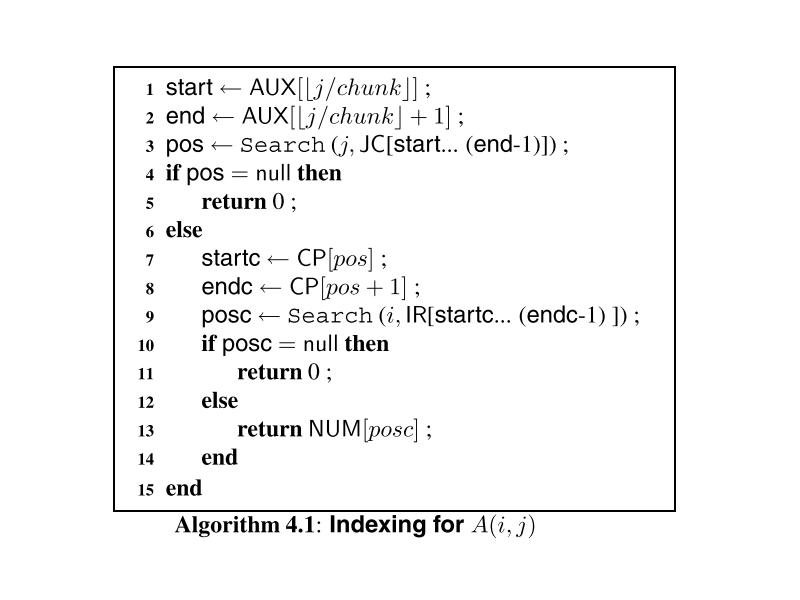
\includegraphics[scale=0.4]{index.png}
\end{center}
\end{frame}

\begin{frame}[fragile]{Illustration of Indexing}
	\begin{columns}
\begin{column}{0.5\textwidth}
  \centerline{Matrix A} \\
   \begin{blockarray}{ccccccc}
	\hspace{1cm} & 0 & 1 & 2 & 3 & 4 & 5 \\
\begin{block}{c(cccccc)}
  0 & 0 & 1 & 0 & 0 & 0 & 0\\
  1 & 0 & 0 & 0 & 0 & 0 & 0\\
  2 & 0 & 0 & 3 & 0 & 0 & 0\\
  3 & 0 & 2 & 0 & 0 & 0 & 0\\
  4 & 0 & 0 & 0 & 0 & 0 & 0\\
  5 & 0 & 0 & 0 & 0 & 0 & 4\\
\end{block}
\end{blockarray}
Search for A(i,j) = A(2,2)
\end{column}
\begin{column}{0.5\textwidth}  %%<--- here
\begin{center}
\begin{comment}
	NUM = [1, 2, 3, 4] \\
    IR  = [0, 3, 2, 5] \\
    CP = [0, 2, 3, 4] \\
    JC = [1, 2, 5] \\
	AUX = [0, 2, 3, 4] \\
\end{comment}
	n = 6, nnz = 4, nzc = 3 \\
	$\ceil{cf} = n+1/nzc = \ceil{2.33}$ \\
	
	$\highlight{\therefore \ceil{cf} = 3}$ \\
	\vspace{0.2cm}
	Let $s = \floor{j/cf} = \floor{2/3} = \floor{0.66} $
	$\highlight{\therefore s = 0}$
\end{center}
	
\end{column}
\end{columns}
\end{frame}

\begin{frame}[fragile]{Illustration of Indexing}
	\begin{columns}
\begin{column}{0.5\textwidth}
  \centerline{Matrix A} \\
   \begin{blockarray}{ccccccc}
	\hspace{1cm} & 0 & 1 & \highlight{2} & 3 & 4 & 5 \\
\begin{block}{c(cccccc)}
  0 & 0 & 1 & \highlight{0} & 0 & 0 & 0\\
  1 & 0 & 0 & \highlight{0} & 0 & 0 & 0\\
  2 & 0 & 0 & \highlight{3} & 0 & 0 & 0\\
  3 & 0 & 2 & \highlight{0} & 0 & 0 & 0\\
  4 & 0 & 0 & \highlight{0} & 0 & 0 & 0\\
  5 & 0 & 0 & \highlight{0} & 0 & 0 & 4\\
\end{block}
\end{blockarray}
Search for A(i,j) = A(2,2)
\end{column}
\begin{column}{0.5\textwidth}  %%<--- here
\begin{center}
\begin{comment}
	NUM = [1, 2, 3, 4] \\
    IR  = [0, 3, 2, 5] \\
    CP = [0, 2, 3, 4] \\
    
\end{comment}
	AUX = [0, 2, 3, 4]\\
	AUX[0] = 0 and AUX[0+1] = 2 \\
	Search JC[0...(2-1)] = {1,2} for j=2 \\
	where JC = [1, 2, 5] \\
	Found! \\
	$\therefore$ pos = index of JC where j found \\
	pos = 1 \\
\end{center}
	
\end{column}
\end{columns}
\end{frame}

\begin{frame}[fragile]{Illustration of Indexing}
	\begin{columns}
\begin{column}{0.5\textwidth}
  \centerline{Matrix A} \\
   \begin{blockarray}{ccccccc}
	\hspace{1cm} & 0 & 1 & 2 & 3 & 4 & 5 \\
\begin{block}{c(cccccc)}
  0 & 0 & 1 & 0 & 0 & 0 & 0\\
  1 & 0 & 0 & 0 & 0 & 0 & 0\\ 
  \highlight{2} & \highlight{0} & \highlight{0} & \highlight{3} & \highlight{0} & \highlight{0} & \highlight{0}\\
  3 & 0 & 2 & 0 & 0 & 0 & 0\\
  4 & 0 & 0 & 0 & 0 & 0 & 0\\
  5 & 0 & 0 & 0 & 0 & 0 & 4\\
\end{block}
\end{blockarray}
Search for A(i,j) = A(2,2)
\end{column}
\begin{column}{0.5\textwidth}  %%<--- here
\begin{center}
\begin{comment}
	NUM = [1, 2, 3, 4] \\
\end{comment}
	Let sc = CP[pos] \\
	where CP = [0, 2, 3, 4] \\
	CP[1] = 2 and CP[1+1] = 3 \\
	Search IR[2...(3-1)] = {2} for i=2 \\
	where IR  = [0, 3, 2, 5] \\
	Found! \\
	$\therefore$ pos = index of IR where i found \\
	posc = 2 \\
\end{center}
	
\end{column}
\end{columns}
\end{frame}
\begin{frame}[fragile]{Illustration of Indexing}
	\begin{columns}
\begin{column}{0.5\textwidth}
  \centerline{Matrix A} \\
   \begin{blockarray}{ccccccc}
	\hspace{1cm} & 0 & 1 & \highlight{2} & 3 & 4 & 5 \\
\begin{block}{c(cccccc)}
  0 & 0 & 1 & 0 & 0 & 0 & 0\\
  1 & 0 & 0 & 0 & 0 & 0 & 0\\ 
  \highlight{2} & 0 & 0 & \highlight{3} & 0 & 0 & 0\\
  3 & 0 & 2 & 0 & 0 & 0 & 0\\
  4 & 0 & 0 & 0 & 0 & 0 & 0\\
  5 & 0 & 0 & 0 & 0 & 0 & 4\\
\end{block}
\end{blockarray}
Search for A(i,j) = A(2,2)
\end{column}
\begin{column}{0.5\textwidth}  %%<--- here
\begin{center}
\begin{comment}
	
\end{comment}
	NUM[posc] = NUM[2] \\	
	where NUM = [1, 2, 3, 4] \\	
	$\therefore$ value at A(2,2) = 3\\
\end{center}
	
\end{column}
\end{columns}
\end{frame}

\begin{frame}{Complexity of Search}
\begin{enumerate}
	\item The expected cost of column-wise indexing is constant assuming that nonzero columns (columns that contain at least one nonzero) are distributed evenly.
	\item Worst-case performance of column-wise indexing is $log_{10} \ceil{cf}$
\end{enumerate}
	
\end{frame}



\begin{frame}{References}
	[1] Buluc, A., \& Gilbert, J. R. (2008). On the Representation and Multiplication of Hypersparse Matrices. https://doi.org/10.1109/IPDPS 2008.4536313
\end{frame}

\end{document}
